\section{Background} \label{sec:background}
%\subsection{Low-code Software (LCS) Development and Phases}\label{sec:background-lcsd}
\nd\bf{What is an  Low-code Application?} To cater to the demand of the competitive market, business organizations often need to quickly develop and deliver customer-facing applications.  LCSD platform allows the quick translation of the business requirement into a usable software application. It also enables citizen developers of varying levels of software development experience to develop applications using visual tools to design the user interface in a drag-and-drop manner and deploy them easily~\cite{lowcodewiki}.  LCSD is inspired by the model-driven software principle where abstract representations of the knowledge and activities drive the development, rather than focusing on algorithmic computation~\cite{sahay2020supporting}.  LCSD platforms aim to abstract away the complexity of testing, deployment, and maintenance that we observe in traditional software development. Some of the most popular low-code platforms are Appian~\cite{appian}, Google App Maker~\cite{googleappmaker}, Microsoft Powerapps~\cite{powerapps}, and Salesforce Lightning~\cite{salesforce}. 
%Rapid development in traditional software development is facilitated by the reuse of software libraries like APIs. Like traditional software,  LCSD platforms also offer APIs that can be reused by other  LCSD platforms or software.  

% \nd\bf{APIs in Low-code.} API (Application Programming Interface) is an interface that allows seamless information exchange between multiple systems. It defines how data will be exchanged so that different applications can use this interface independently \cite{uddin2012temporal}. However, the design and maintenance of an efficient API requires a team of expensive experienced developers. LCDPs provide user-friendly interfaces to integrate third party APIs and expose APIs for others to consume by abstracting away the complexity of data modeling, server maintenance, scalability issues.
%\anindya{Alamin, check if no sentence is copied from any source in the paras above or below. If you are inspired by some discussion, you have to paraphrase it.}

% visual tools to quickly define and build UI and forms. but visual tools like data models, workflows are becoming popular.
% Instead of coding the application non-technical people can assemble an application.
% Build application with appropriate modules and use appropriate data storage.
% and it is cloud and platform agnostics
% No universal standard yet.

%\subsection{Development Stages of Low-code Application}
%\anindya{The para below is commented as it is repetition of previous discussion.}
%Low-code software development is bringing in digital transformation to commercial applications as well as softwares for internal usage. It handles lots of software development, deployment, and maintenance challenges. It does not replace the traditional software development, rather supplements it by addressing the high demand for different types of software vs the talent gap by reducing the entry-level barrier for people without a strong programming background. Traditional software expertise is required for complex application development, because debugging and fixing deployment issues are quite challenging.


\begin{figure}[t]
\centering
% 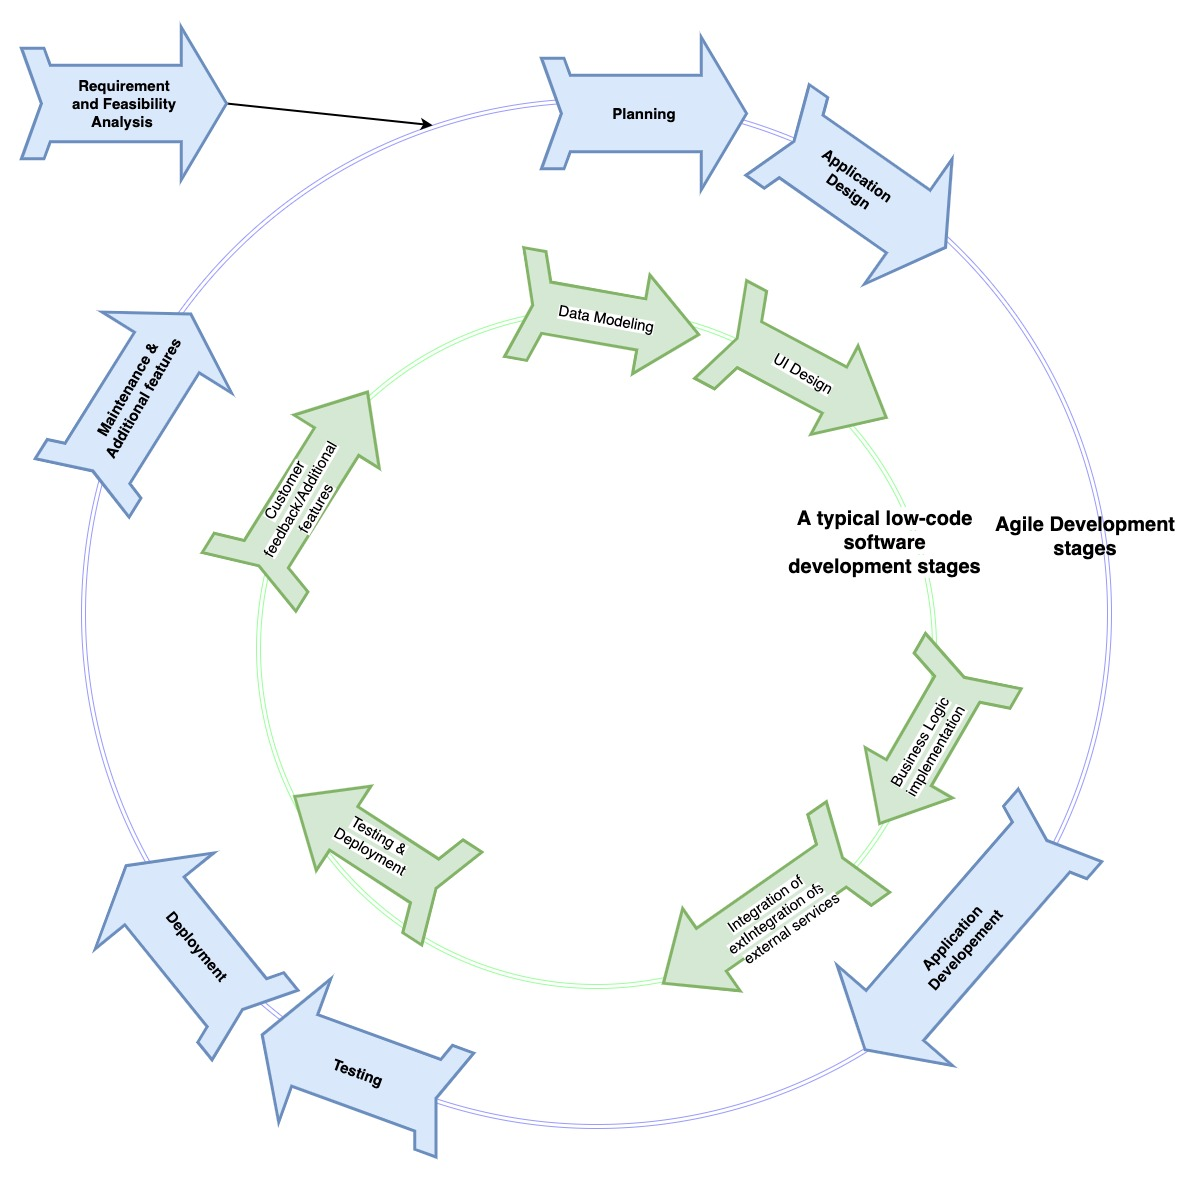
\includegraphics[scale=.22]{res/development_flow-Page-agile_lc.jpg}
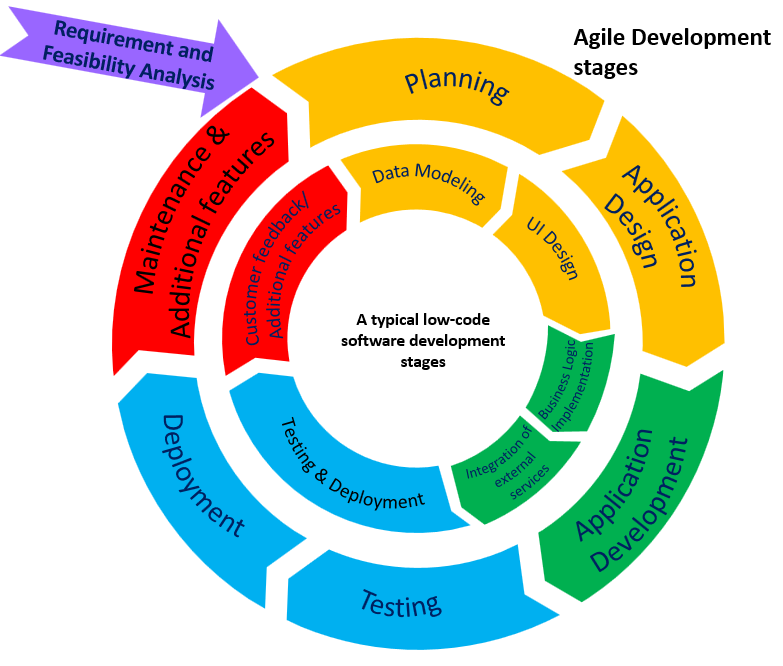
\includegraphics[scale=.50]{res/development_cycle.PNG}
% 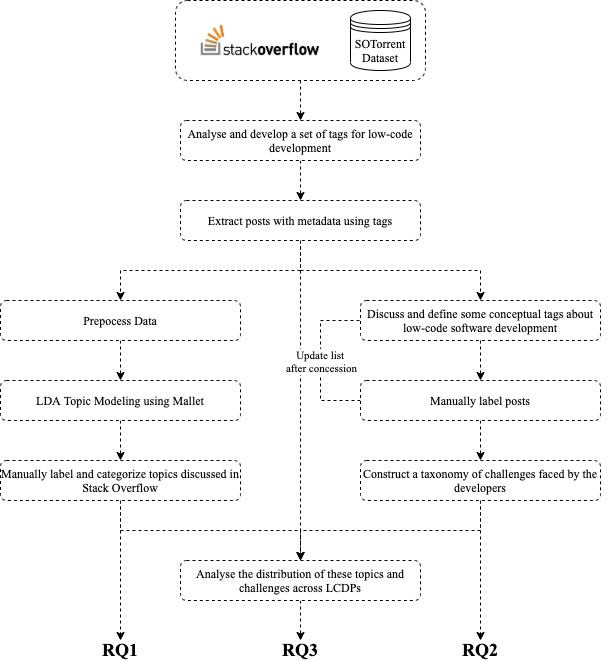
\includegraphics[width=0.35 * linewidth]{res/methology_overview.jpg}
\caption{Agile methodologies in traditional vs  LCSD development}
\label{fig:low-code-agile}
\vspace{-5mm}
\end{figure}

\nd\bf{Development Phases of an  LCSD Application.} A typical  LCSD application can be built in two ways~\cite{sahay2020supporting}: \begin{inparaenum}
\item ``UI to Data Design'', where developers create UI and then connect the UI to necessary data sources, or \item ``Data to UI'' where the design of the data model is followed by the design of the user interfaces. \end{inparaenum} In both approaches, application logic is implemented, and then third party services and APIs are integrated. APIs are interfaces to reusable software libraries~\cite{Robillard-APIProperty-IEEETSE2012}.  
% Application monitoring dashboard, server maintenance, scaling up, etc., are usually supported by the  LCSD platforms. 
A major motivation behind  LCSD is to build applications, get reviews from the users, and incorporate those changes quickly~\cite{waszkowski2019low-automating}. As such, the agile development methodology~\cite{beck2001manifesto} and  LCSD can go hand in hand because the fundamental principle and objective are customer satisfaction and continuous incremental delivery. The inner circle of Figure~\ref{fig:low-code-agile} shows the important development phases of an  LCSD application, as outlined in~\cite{sahay2020supporting}. The outer circle of \fig\ref{fig:low-code-agile} shows the phases in a traditional agile software development environment. As  LCSD platforms take care of many of the application development challenges, some of the agile application development phases have shorter time/execution spans in  LCSD compared to traditional software development. 
%(see \fig\ref{fig:low-code-agile}). 




% \bf{Agile development methodology in low-code application life cycle.}


%\section{Related Work} \label{sec:related_work}


 
%  \subsection{Topic modeling in Software Engineering Research}

% Barua et al.\cite{barua2014developers} conducted a study using LDA topic modeling to gain insightful information regarding developers community and how topics evolve over time in different software domains.
% Rosen et al. \cite{rosen2016mobile} use topic modeling of discussions in Stack Overflow and present popular, difficult topics on mobile development. Yang et al. use topic modeling with ML algorithm to find popular and difficult security topics and categorized them into 5 topics \cite{yang2016security}. Bajaj et al.  \cite{bajaj2014mining} used unsupervised learning to categorize important web development topics, common misconceptions,  and shared and overview of how these questions are evolving over time. Bagherzadeh \& Raffi \cite{bagherzadeh2019going} studied what big data developers asks in SO and their challenges. Adrian et al. used topic modeling on source code to find linguistic topic to find the intention of the code and how these topics are distributed over the system \cite{kuhn2007semantic}. 

% 

%\subsection{Exploratory Study Using SO data}